\documentclass[twoside]{article}
\usepackage[utf8]{inputenc}
%\usepackage[uebung, answers]{tumbgdm}
\usepackage[uebung]{tumbgdm}
\usepackage{lecturesetup}
\nummerUebungsblatt{3}
\nummerErsteFrage{6}

\LearningOutcome{
  You practice some aspects of Turing machines, you learn how nested loops can be used to find permutations,
  you learn how least-squares problems are solved in MATLAB, and you optionally see a story for a real-world
  application of this principle in GNSS (Global Navigation Satellite Systems, for example GPS, GLONASS, or the European Galileo) and other distance-based positioning systems. 
}

\begin{document}
\maketitle


\begin{task}{Turing Machine}{}{}
The Lecture introduced Turing Machines and how to write programs for
them. In this task we will practice to implement some simple turing
machines.
\begin{enumerate}
\item{\textbf{Even Number:} Create a Turing Machine that accepts all even numbers. Remember that a Turing machine accepts a language (e.g., set of strings) if the machine terminates for all of them in a accepting state. You can declare any state to be accepting, introduce maybe two states \code{accept} and \code{reject} and let the Turing machine go into \code{accept} for even numbers and into \code{reject} for uneven numbers.
  Tip: Formulate the machine with pen and paper. This is what you need to learn. Only after formulating the machine, feel free to test it, for example on \url{https://www.turingmachine.io/}}
  

  \item{\textbf{Even Numbers with Result on Tape:}
  Create a Turing Machine that accepts all even numbers and writes \(\epsilon \; N \epsilon\) for uneven or
  \(\epsilon \; Y\epsilon\) for even numbers. If you did not find a solution for the previous tasks, write
  two Turing machines: both start out by clearing the current word on tape (walk right until you find an empty, walk left writing emtpy until you find an empty. The first machine, then writes 'Y' onto the tape, the second one 'N'. 
  }

  \item{\textbf{Unary Addition:}
    Create a Turing Machine that adds two numbers given as a string \code{III+II} on the tape. Make sure that the Turing machine ends on the beginning of the result. Note that the solution can be rather simple.
  }

  \item{\textbf{Doubling Chars:}
    Create a Turing Machine that doubles every occurence of the letter \code{a} on a tape. }

\item{\textbf{Reversing:} Create a Turing Machine that reverses the contents of a tape. By this, we mean that the result consists of the same characters in the opposite order.
}
  \end{enumerate}

\begin{solution}
  The following snippets for \url{https://www.turingmachine.io} solve the problems.

  \begin{enumerate}
  \item{\textbf{Unary Addition:}

    \begin{lstlisting}
    # Unary Addition - A rather simple trick
blank: ' '
start state: search
input: 'III+II'
table:
  search:
    1: {write: 0, R: search}
    0: {write: 1, R: search}
    +: {write: ' ', R: done}
  done:

    \end{lstlisting}
    

    }
  \end{enumerate}

  
\end{solution}


\end{task}




\begin{task}{Permutations}{}{}

Sometimes we need to look at different combinations of a set of inputs.
This means we need to generate all possible permutations of an input
set.

\begin{enumerate}
\item{\textbf{Permutations of 3 Numbers:} Given a vector with 3 different numbers
  like \code{[1,2,3]} write a MATLAB program that generates all possible permutations into a new
  matrix each permutation on a new row. The output should be a matrix with three columns
and each row being a different permutation, that is, similar to
\code{ [[3, 2, 1]; [2, 3, 1]; [2, 1, 3]; [3, 1, 2]; [1, 3, 2]; [1, 2, 3]]}.
}
\item{\textbf{Permutation of a vector:} Extend the previous program to create all permutations of a vector of 4 values.}
\end{enumerate}

\end{task}

 
%\hypertarget{task-7-permutations}{%
%  \section{Task 7: Permutations}\label{task-7-permutations}}
%

\begin{task}{Method of Least Squares\up*}{}{}
When working with measurements from the real world errors are
unavoidable. These errors can often be reduced by using multiple
measurements. Since these measurements will contradict each other we
need a method to resolve this contradiction.

Assuming, that the relationship between measurements and the actual
values, we can create the system of overdetermined linear equation

\[
Ax = b
\] where \(b = (b_1,\ldots,b_n)\) contains the measurements, \(x\)
the actual value we want to infer and \(A\) expresses the
\emph{theoretic} relationship between them. We also assume that \(A\)
has maximal rank, meaning that the column vectors of \(A\) are linearly
independant. Because the perfect solution for \(x\) does not exist, due
to the errors in measurement, we are looking for the value of x which
minimizes the \emph{norm} of the residium \(r(x)\):

\[
\sqrt{\sum_{i=1..n}{r_i^2}} = ||\begin{pmatrix}r_1\\...\\r_i\\...\\r_n\end{pmatrix}||=||r(x)|| = ||b-Ax||\]

A perfect solution would be a a \emph{norm} of zero. For the Euclidian
norm we can simplify the term by squaring both sides, as the norm is
defined as the square root of the scalar product, therefore a minimal
norm corresponds to a minimal scalar product. We can formulate the
following equation:

\[ || r(x) || ^2 =(b-Ax)^T(b-Ax) = x^T A^T Ax - 2x^T A^T b + b^T b \rightarrow min\]

As we want to find the minimum we can use differential calculus and set
the first derivative to zero:

\[\frac{\partial}{\partial x} ||r(x)||^2 = 2A^T Ax - 2 A^T b = 0\]

This equation is called \emph{normal equation of an overdetermined
  system of linear equation} \(Ax=b\) and is usually given in the
equivalent form:

\[A^T Ax = A^T b\]

\(A^T A\) is a positive semi-definite, \textbf{symmetric} matrix. As a
result the equation can easily be solved for \(x\) as it is not
overdetermined anymore. This \(x\) minimizes the error function norm.
The Gauss-Markov theorem actually proves that this algorithm provides a
best, linear, unbiased estimate value of \(x\). Which is in asense the
most probable value of \(x\) given the set of measurements.

\begin{enumerate}
\item{
  Using the measured values \code{b = [14.1000;25.9000;18.0500;41.9500]} and a matrix of
  \code{A = [1,2,3;4,5,4;6,3,2;7,7,7]}, calculate the normal equation in MATLAB. Note that matrix transposition is available
  in MATLAB either as a symbol like in \code{A'} or as a function like \code{transpose(A)}.
}
\item{
Solve the normal equation set up in the previous task with MATLAB. Note that it is not good practice to compute the inverse of the matrix $A$, as its realization in main memory can produce fatal rounding errors. It is better to recall the right division in MATLAB from a previous sheet.
  }
\item {
  As the equation is overdetermined, the solution will not be exact. Compute the vector of residual values
  \[
     r = b-Ax
     \]
     and its size
     \[
     ||r||
     \]
     For the size, consider using the MATLAB function \code{norm}.
  }

    
  \end{enumerate}
\end{task}

\begin{task}{Lateration\up{+}}{}{}
Follows.
\end{task}
Lateration is a technique for deriving the location of a point in space
by measuring the distance to a number of points, whose location is
known. This technique is used in GNSS systems including GPS, Galieo, or GLONASS
where the distance is measured by signal travel time. Note that in these cases,
in addition to the three unknown coordinates, there is a fourth one representing a
very accurate time. More information on this can be found by searching for Time-of-Arrival
on the Internet.

\begin{center}
  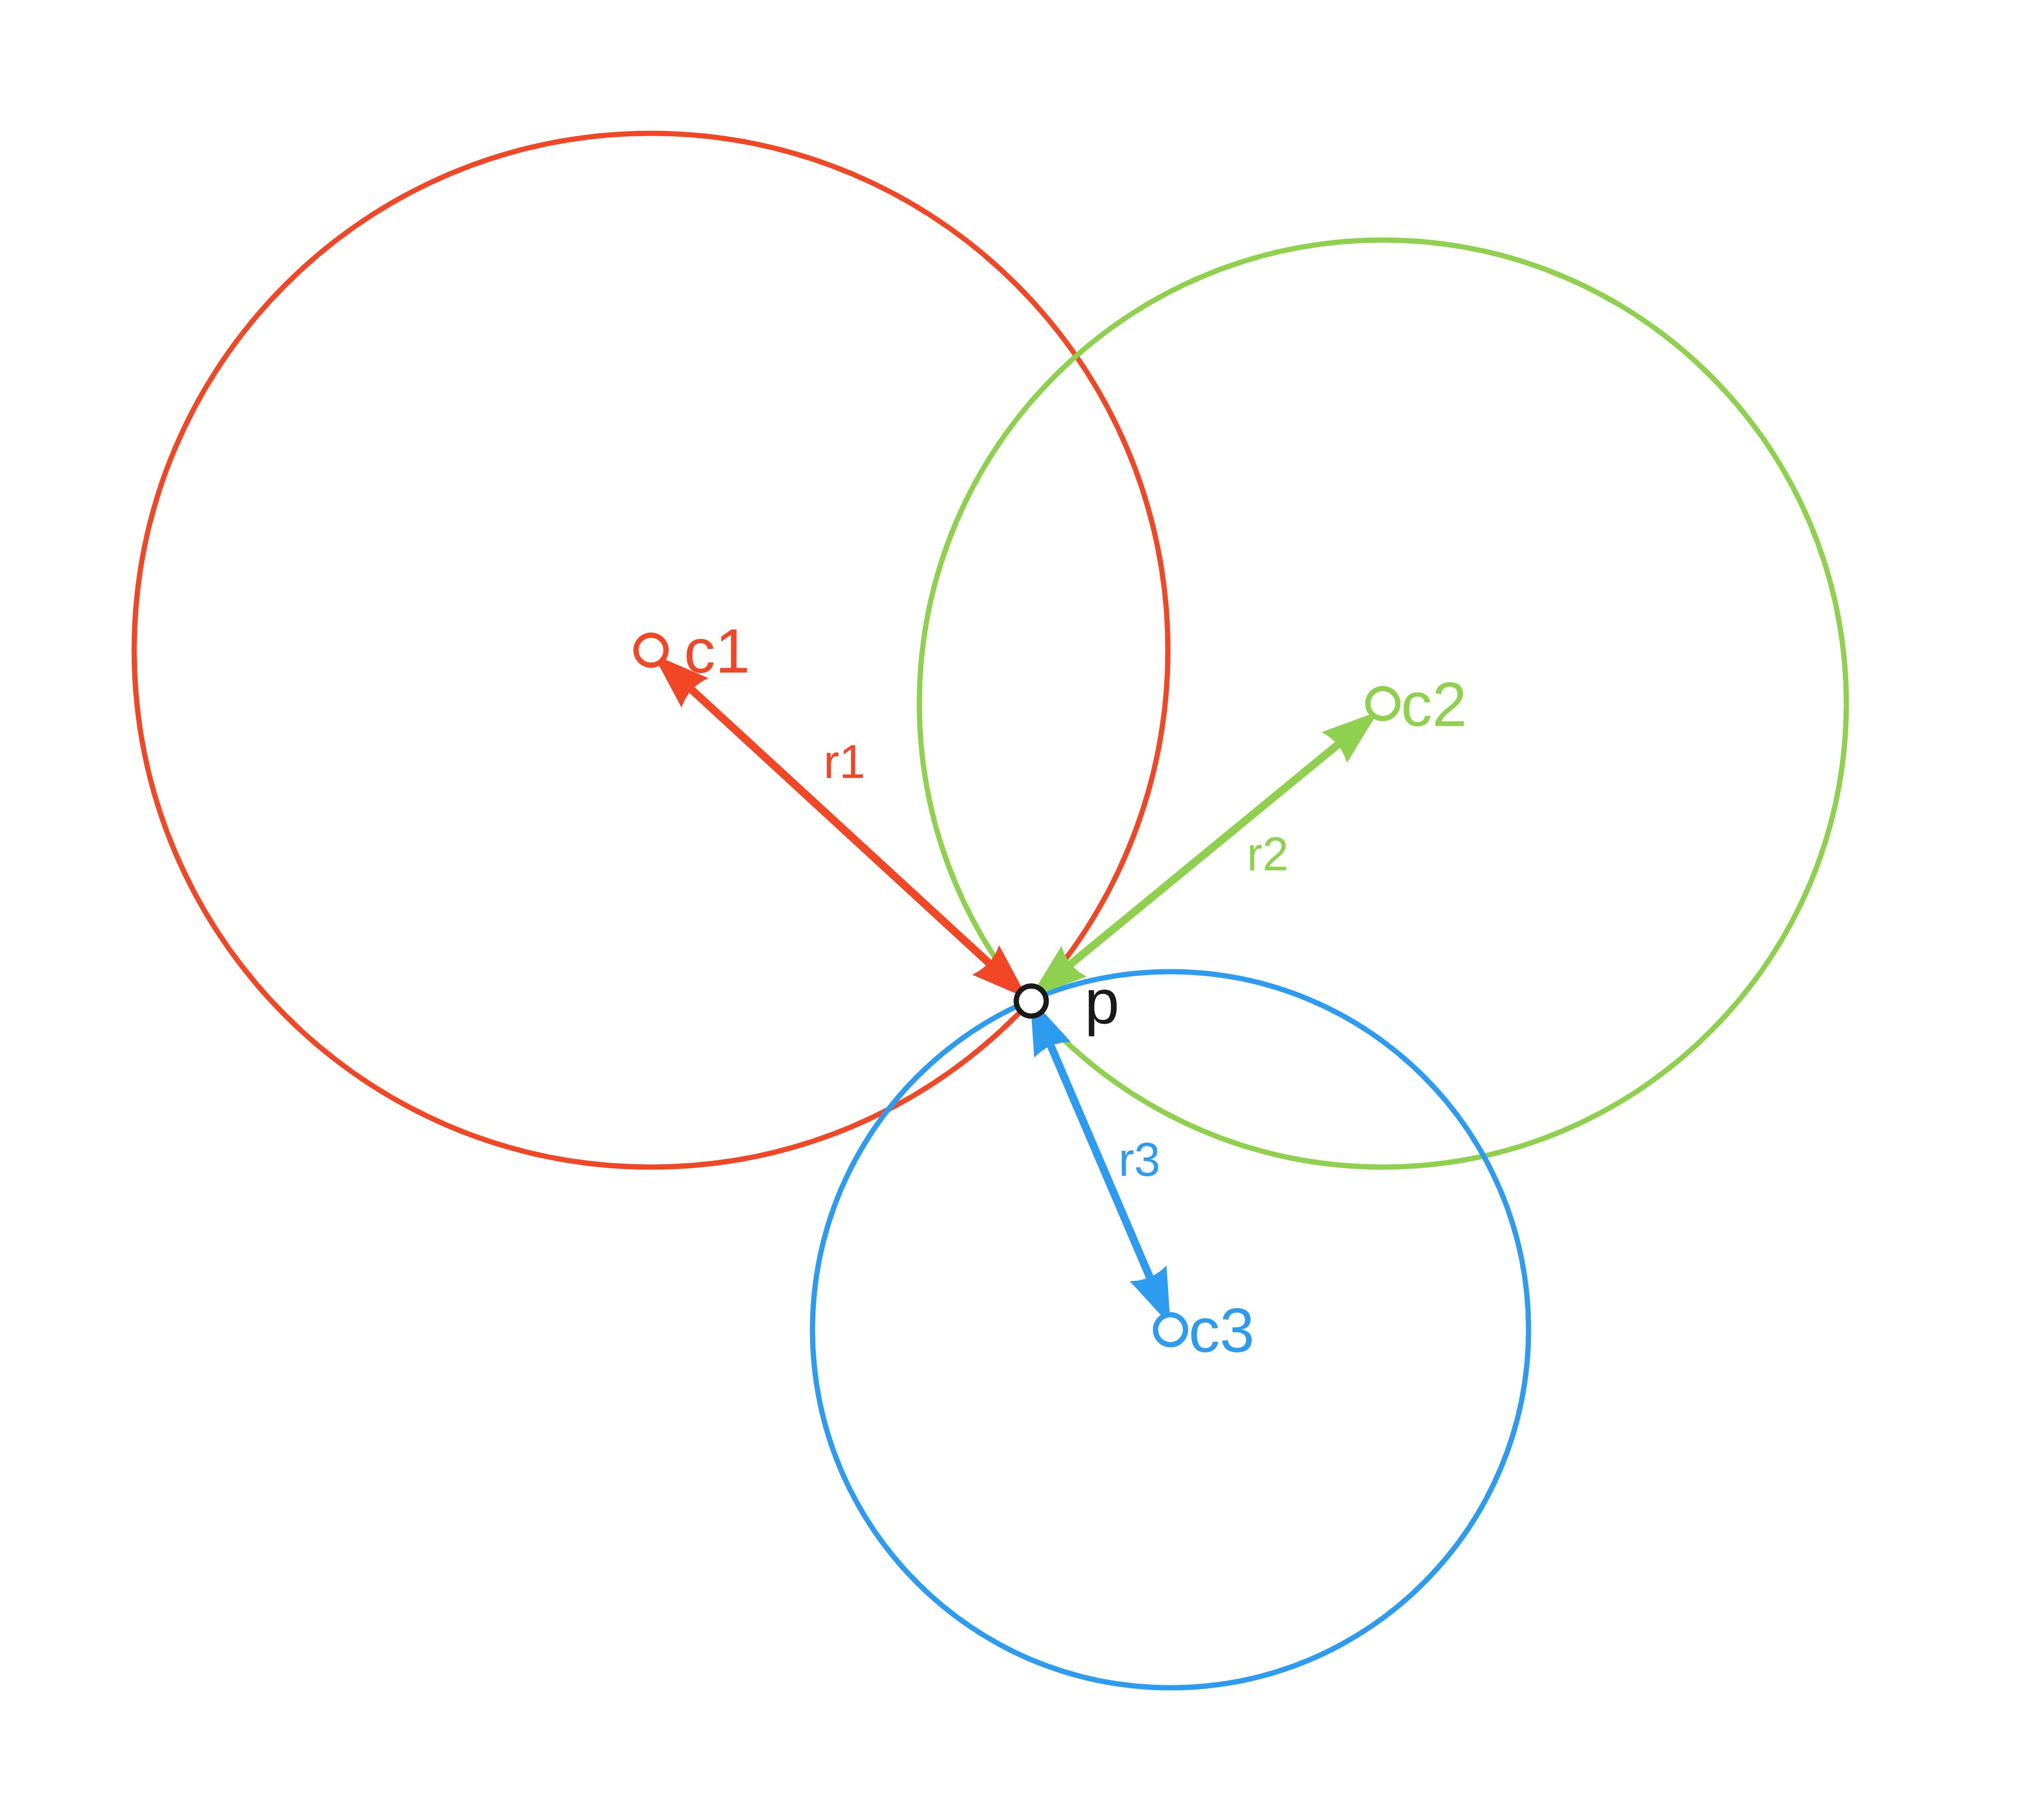
\includegraphics[width=10cm]{gfx/2021_09_laterationsetup.png}
\end{center}
Here \(c_1\), \(c_2\), and \(c_3\) are the the known positions with the
measured radii \(r_1\), \(r_2\), and \(r_3\) And \(p\) is the point we
are looking for.

Put formally the location \(p = (x,y)\) must fulfill all equations
\(k_i\) describing circles around the known centers \(c_i = (x_i, y_i)\)
with measured radii \(r_i\):

\[r_i = k_i(x,y) = \sqrt{(x_i-x)^2 + (y_i-y)^2} i = 1..k\]

This is a
nonlinear problem and therefore the least squares algorithm can not be
used directly. Instead we can use an iterative approach based on
starting with a coarse estimation of the location \(p\). Then we can use
the taylor approximation to linearize the system of equations. This
linearization is only valid around the previous location and can be
solved using the least squares algorithm. The linearization is based on
the following Taylor expansion:

\[
  f(x) = \sum_{i=1..n}{ \frac{f^{i}(x_0)}{i!}(x-x_0)^i + R_{n+1}(x,x_0)}
\]

Here, the Term \(R\) collects the remaining error of using a finite sum.
In order to linearize a system of equations using Taylor expansion, we
can set \(n=1\) and ignore \(R\). For our case of lateration, we need
the partial derivatives in both directions to construct the Taylor sum
as a vector expression. These partial derivatives are given as follows:
\[
  \frac{\partial}{\partial x} k_i(k,y) = - \frac{x_i-x}{\sqrt{(x_i-x)^2+ (y_i -y)^2}}
\]
\[\frac{\partial}{\partial y} k_i(k,y) = - \frac{y_i-y}{\sqrt{(x_i-x)^2+ (y_i -y)^2}}\]

Let now \((\tilde{x}, \tilde{y})\) denote the current estimate of the
location \(p\), then using the measurements \(r_i\) we are left with the
following system of linear equations:

\begin{equation}\label{eq:1}
  r_i = k_i(\tilde{x}, \tilde{y}) + \frac{\partial}{\partial x} k_i(\tilde{x}, \tilde{y})(x - \tilde{x}) + \frac{\partial}{\partial y} k_i(\tilde{x}, \tilde{y})(y - \tilde{y}) i \;= \;1..k
\end{equation}
Introducing the notation \(\hat{x}=x-\tilde{x}\) and
\(\hat{y}=y-\tilde{y}\), we get an overdetermined system of linear
equations for which the least squares method can be applied directly.
This results in a vector expressing a correction of the current location
estimate \((\hat{x}, \hat{y})\) this can be added to the the last
location estimate and the process can be iterated.

\begin{enumerate}
   \item{\textbf{Simple Form of Equation:} Use the values from below and fill in Eqation (\ref{eq:1}). bring it to the
     form \(Ax=b\). What are the values of \(A\) and \(b\)? \newline \emph{When looking closely, you will see that when putting in the constant values for the measurements and the known locations into Equation \ref{eq:1} that only two variables remain. These form together the vector $x = (\hat x, \hat y)$ you want to solve for. The solution is \textbf{not} the location we are after, but due to $\hat x = x - \tilde x$ an offset to improve the current location estimate $\tilde x$ (same for y)}}
   \item{\textbf{Program the Matrix and Constants:} Implement the following procedures:
\begin{lstlisting}[language=MATLAB]
function ret = get_A(tilde_x, tilde_y, C, r)

end

function ret = get_b(tilde_x, tilde_y, C, r)

end
\end{lstlisting}
In this context, the matrix C will hold the known locations, $r$ the measured radii:

\[C= \begin{pmatrix}x_1\;y_1\\x_2\;y_2\\x_3\;y_3\\x_4\;y_4\end{pmatrix}=\begin{pmatrix}0\;0\\10\; 0\\15\;0\\0\;12\end{pmatrix} \;\;  \;\;r = \begin{pmatrix}r_1\\r_2\\r_3\\r_4\end{pmatrix}=\begin{pmatrix}2.92\\8.14\\15.46\\9.89\end{pmatrix}\]
Feel free to simplify the signature by removing parameters you don't need.
   }
   \item{\textbf{Location Estimation:}
Given the previously mentioned set of locations and measurements calculate the
estimated location correction in each step, starting with the initial
location estimate \((\tilde{x},\tilde{y}) =(20,20)\). Report this vector for at least 3 steps.
Then run the program for seven steps and report the final result. Try to implement a version with a \code{while} loop
that stops as soon as the error (as measured by the residuum) does not decrease enough.
   }
\end{enumerate}







\end{document}
